\section{Bezier}

Uma curva Bézier pode ser definida por um qualquer numero de pontos, pontos
estes chamados pontos de controlo da curva. Transformações como translação
e rotação podem ser aplicadas na curva manipulando estes pontos. 

O algoritmo de Casteljeau oferece uma construção geométrica de onde se pode
dividir uma curva de Bézier em duas curvas Bézier num parâmetro arbitrário t [0,1]. Como se pode observar:

\begin{center}
 	
 	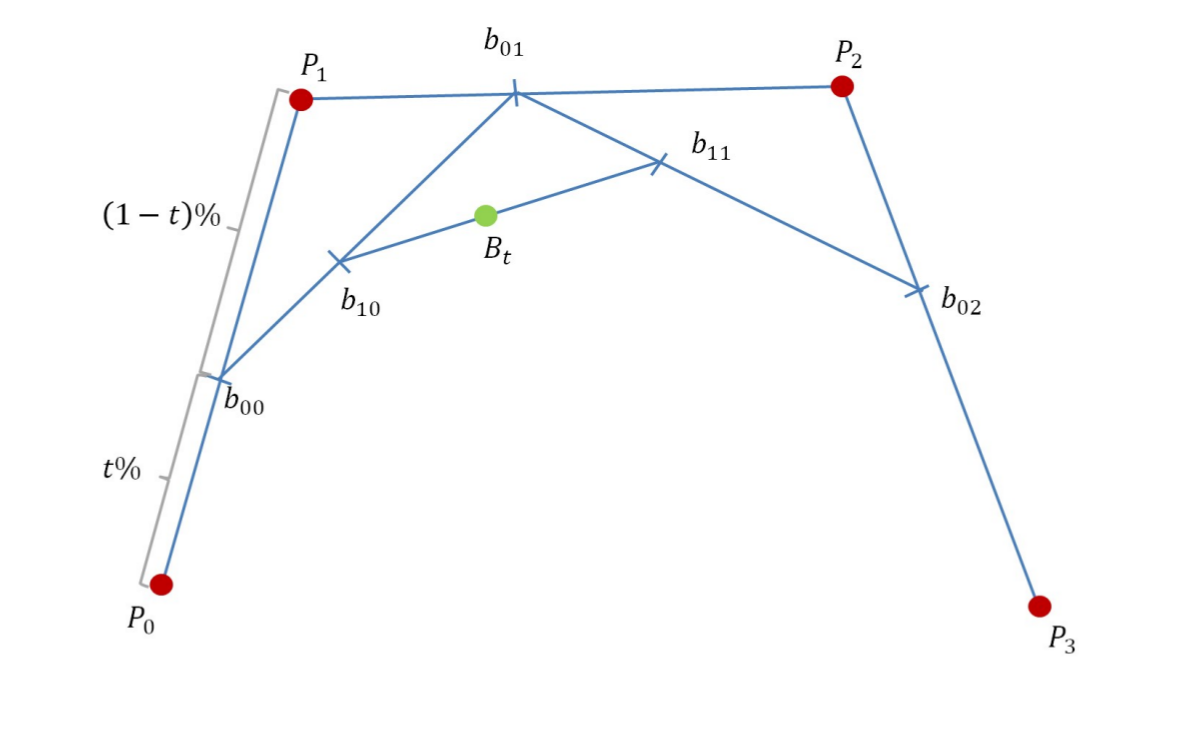
\includegraphics[scale=0.7,keepaspectratio]{resources/casteljou.png}
 	\captionsetup{type=figure, width=0.8\linewidth}
	\caption{Algoritmo geométrico Casteljeau}
\label{fig:ssec1:diagram:plane:to:sphere} 
\end{center}

Fazendo os cálculos manualmente 
\begin{center}
 	
 	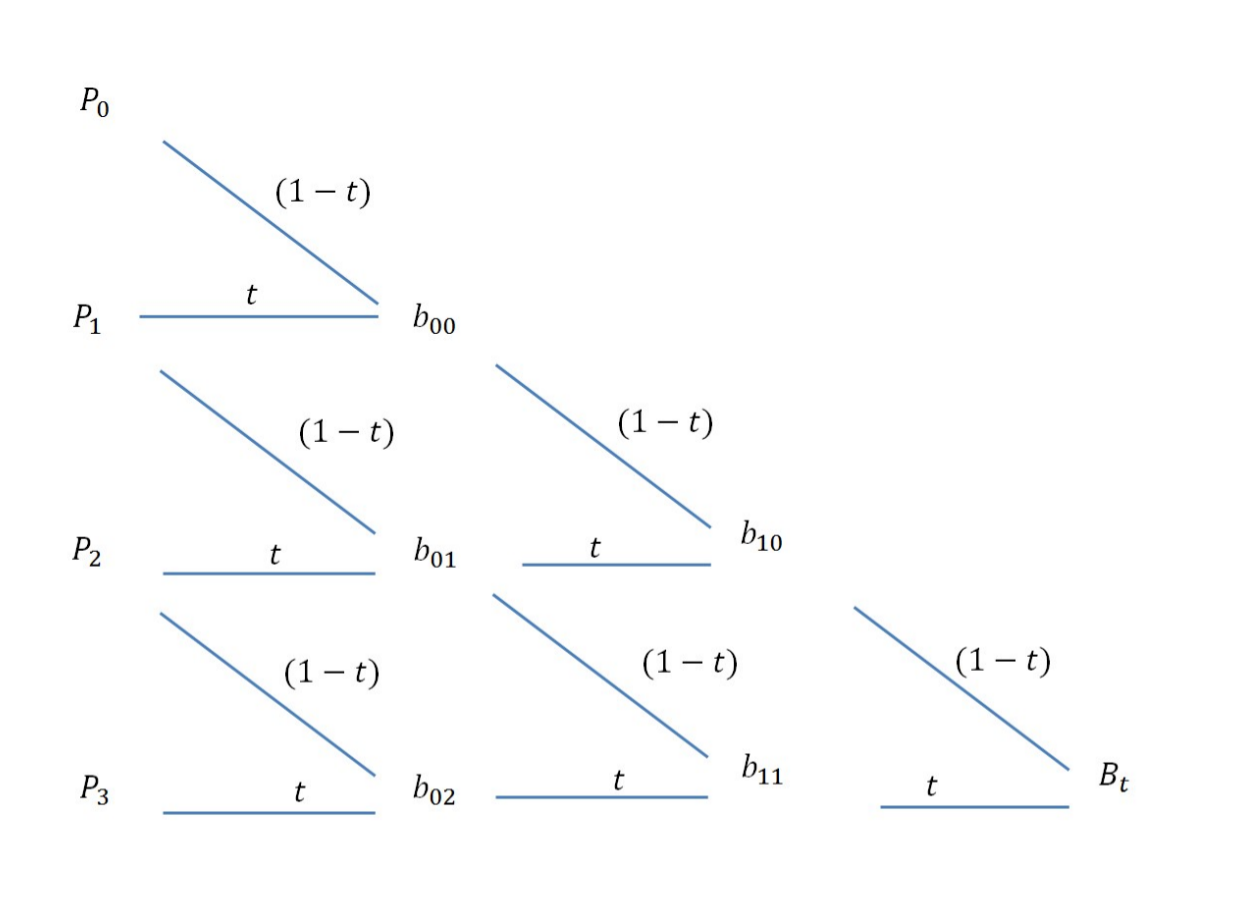
\includegraphics[scale=0.7,keepaspectratio]{resources/casteljeau2.png}
 	\captionsetup{type=figure, width=0.8\linewidth}
	\caption{Representação da árvore casteljeau}
\label{fig:ssec1:diagram:plane:to:sphere} 
\end{center}

Para demonstrar estas transformações segue-se o exemplo de uma curva de Bézier
cúbica, isto é, uma curva definida por 4 pontos de controlo:

\begin{center}
 	
 	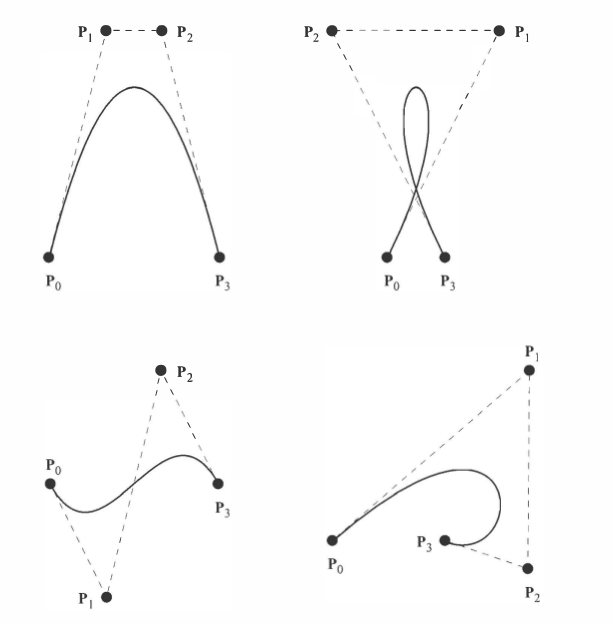
\includegraphics[width=\textwidth,height=\textheight,keepaspectratio]{resources/exemplos1Bezier.png}
 	\captionsetup{type=figure, width=0.8\linewidth}
	\caption{Curvas exemplo de Bézier}
\label{fig:ssec1:diagram:plane:to:sphere} 
\end{center}

Como se pode observar cada uma das curvas observadas possui 4 pontos de
controlo, $P_0$, $P_1$, $P_2$ e $P_3$. A figura demonstra alguma das formas que
uma curva de Bézier pode tomar. 
As curvas de Bézier, independentemente do número de pontos de controlo que
possam ter, são sempre definidas pela seguinte fórmula:
\begin{equation}
B(t)=\sum_{k=0}^{n}B_{n,k}(t)P_{k}
\end{equation}

onde n corresponde a ($nº pontos de controlo - 1$), e 
$t \in [0,1]$ e o seu somatório é sempre igual a 1.




Com 4 pontos de controlo, uma curva de Bézier diz-se cúbica e pode ser definida
pela seguinte formula:




\begin{equation}
B(t)=\sum_{k=0}^{3}B_{3,k}(t)P_{k}
\end{equation}

\begin{equation}
B(t)=t^{3}P_{3}+3t^{2}(1-t)P_{2}+3(t(1-t)^{2})P_{1}+(1-t)^{3}P_{0}
\end{equation}

Onde, após cálculos se chegará a:

B(t)=  $\begin{bmatrix}
       t^{3} & t^{2} & t & 1          \\[0.3em]
		\end{bmatrix}$
		$\begin{bmatrix}
		       -1 & 3 & -3  & 1           \\[0.3em]
		        3 & -6 &  3 & 0   \\[0.3em]
		       -3 & 3 & 0 & 0 \\[0.3em]
		       1 & 0 & 0 & 0
		     \end{bmatrix}$
		$\begin{bmatrix}
		       P_{0}           \\[0.3em]
		       P_{1}   \\[0.3em]
		       P_{2} \\[0.3em]
		       P_{3}
		     \end{bmatrix}$


Quanto maior o número de pontos de controlo maior o custo computacional de as representar.

{\huge \textbf{Bezier Patches/superfície:}}

Se se tiver um 2D-\emph{array} de pontos
$P_{i,j}$,$i=0$,$\ldots$,$m$,$j=0$,$\ldots$ $n$, então pode-se
construir uma superfície Bézier da mesma forma que se constrói uma curva Bezier.
Da mesma maneira que nas curvas Bézier, a mais importante e mais usada
é a superfície de Bézier bicúbica (m=n=3) onde é definida por 16 pontos de
controlo $P_{i,j}$ e pode ser escrita da seguinte forma:

\begin{equation}
B(u,v)=\sum_{j=0}^{3}\sum_{i=0}^{3}B_{i}(u)P_{i,j}B{j}(v)
\end{equation}



\begin{center}
 	
 	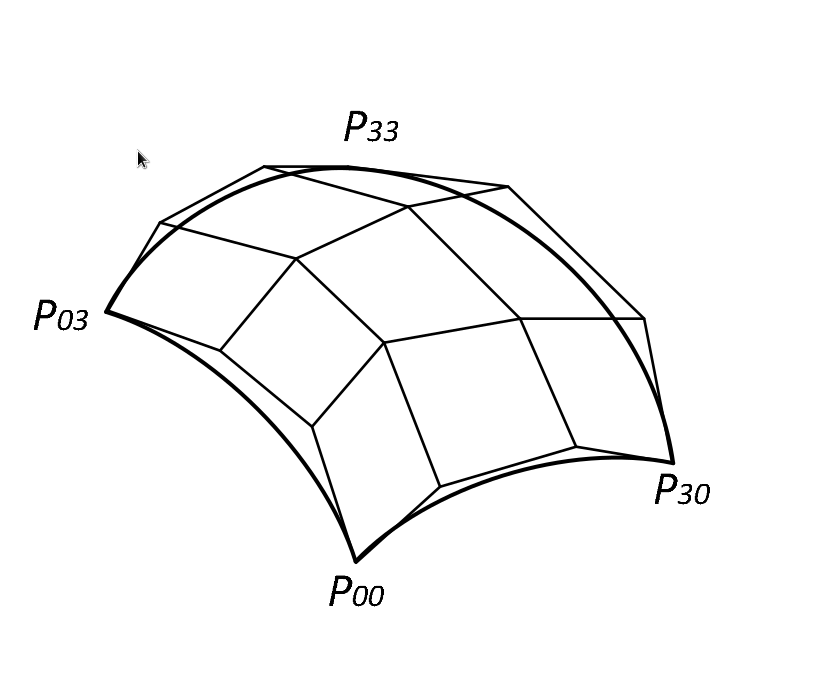
\includegraphics[scale=1,keepaspectratio]{resources/beziersupf.png}
 	\captionsetup{type=figure, width=0.8\linewidth}
	\caption{Superfície de Bézier bicúbica}
\label{fig:ssec1:diagram:plane:to:sphere} 
\end{center}

Sendo U = $\begin{bmatrix}
       u^{3} & u^{2} & u & 1          \\[0.3em]
		\end{bmatrix}$

e M = $\begin{bmatrix}
		       -1 & 3 & -3  & 1           \\[0.3em]
		        3 & -6 &  3 & 0   \\[0.3em]
		       -3 & 3 & 0 & 0 \\[0.3em]
		       1 & 0 & 0 & 0
		     \end{bmatrix}$

Com que foi previamente explicado relativamente às curvas de Bézier, conclui-se
que o método de construção de uma superfície Bézier corresponde a um conjuntos
de curvas de Bézier conjuntas. 
Então:
\begin{equation}
	
	\label{}
\end{equation}
B(u,v) = $\begin{bmatrix}
       u^{3} & u^{2} & u & 1          \\[0.3em]
		\end{bmatrix}$ 
		M$\begin{bmatrix}
		       P_{00} & P_{01} & P_{02} & P_{03}   \\[0.3em]
		       P_{10} & P_{11} & P_{12} & P_{13}   \\[0.3em]
		       P_{20} & P_{21} & P_{22} & P_{23}   \\[0.3em]
		       P_{30} & P_{31} & P_{32} & P_{33}
		     \end{bmatrix}$
		$M^{T} \begin{bmatrix}
		       v^{3}           \\[0.3em]
		       v^{2}   \\[0.3em]
		       v^{1} \\[0.3em]
		       v^{0}
		     \end{bmatrix}$

Este método exato irá ser aplicado mais tarde nos algoritmos.
\section{Splines Catmull-Rom}

A curva de splines Catumull-Rom para dados pontos de controlo $P_{0}, P_{1}, P_{2} e P_{3}$, está definida de modo a que a tangente em cada ponto $P_{i}$ possa ser encontrada através da diferença entre os seus pontos vizinhos $P_{i-1}$ e $P_{i+1}$

\begin{center}
 	
 	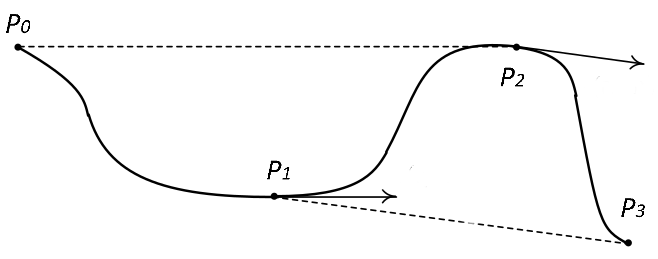
\includegraphics[scale=0.5,keepaspectratio]{resources/catmullDeriv.png}
 	\captionsetup{type=figure, width=0.8\linewidth}
	\caption{Spline Catmull-Rom para os pontos $P_{0}, P_{1}, P_{2} e P_{3}$}
\label{fig:ssec1:diagram:plane:to:sphere} 
\end{center}

Esta curva spline pode ser escrita em forma de matriz:

\begin{equation}
\frac{P_{2}-P_{0}}{2} = P_{1}^{'} = P^{'}(0) = c  \nonumber
\end{equation}
\begin{equation}
P_{1} = P(0) = d 		\nonumber
\end{equation}
\begin{equation}
P_{2}=P(1)=a+b+c+d 		\nonumber
\end{equation}
\begin{equation}
\frac{P_{3}-P_{1}}{2} = P_{2}^{'} = P^{'}(1) = 3a+2b+c 
\end{equation}


o que é equivalante a:

\begin{equation}
P_{0} = a+b-c+d 		\nonumber
\end{equation}
\begin{equation}
P_{1} = P{0} = d 		\nonumber
\end{equation}
\begin{equation}
P_{2}=P(1)=a+b+c+d 		\nonumber
\end{equation}
\begin{equation}
P_{3}=6a+4b+2c+1
\end{equation}

este conjunto de equações pode-se representar na seguinte operação de matrizes:

P=$\begin{bmatrix}
		       P_{0}           \\[0.3em]
		       P_{1}   \\[0.3em]
		       P_{2} \\[0.3em]
		       P_{3}
		     \end{bmatrix}$ = $\begin{bmatrix}
		      					 1 & 1 & -1 & 1           \\[0.3em]
		       					 0 & 0 & 0 & 1   \\[0.3em]
		       					 1 & 1 & 1 & 1 \\[0.3em]
		      					 6 & 4 & 2 & 1
		     					\end{bmatrix}$  $\begin{bmatrix}
		       									a_{x} & a_{y} & a_{z}    \\[0.3em]
		     								  	b_{x} & b_{y} & b_{z}    \\[0.3em]
		       									c_{x} & c_{y} & c_{z}    \\[0.3em]
		       									d_{x} & d_{y} & d_{z} 
		     					\end{bmatrix}$   = $C * A$

Estes cálculos até agora demonstrados irão ser aplicados algoritmicamente no programa da seguinte maneira:

$\begin{bmatrix}
       x(u) & y(u) & z(u)           \\[0.3em]
\end{bmatrix}$ = 
$\begin{bmatrix}
       t^{3} & t^{2} & t & 1          \\[0.3em]
		\end{bmatrix}$ $\begin{bmatrix}
		      					 -0.5 & 1.5 & -1.5 & 0.5           \\[0.3em]
		       					 1 & -2.5 & 2 & -0.5   \\[0.3em]
		       					 -0.5 & 0 & 0.5 & 0 \\[0.3em]
		      					 0 & 1 & 0 & 0
		     					\end{bmatrix}$ $\begin{bmatrix}
         							    P_{0}           \\[0.3em]
       									P_{1}   \\[0.3em]
       									P_{2} \\[0.3em]
       									P_{3}
     \end{bmatrix}$